\documentclass[main.tex,fontsize=8pt,paper=a4,paper=portrait,DIV=calc,]{scrartcl}
% Document
\usepackage[T1]{fontenc}
\usepackage[dvipsnames]{xcolor}
\usepackage[nswissgerman,english]{babel}
\renewcommand{\familydefault}{\sfdefault}

% Format
\usepackage[top=5mm,bottom=1mm,left=5mm,right=5mm]{geometry}
%\setlength{\headheight}{\baselineskip}
%\setlength{\headsep}{0mm}

%\usepackage{scrlayer-scrpage}
%\clearpairofpagestyles
%\chead{{\bfseries\TITLE, \AUTHOR, \pagename~\thepage}}

%\addtokomafont{pagehead}{\upshape}

\usepackage{multicol}
\setlength{\columnsep}{2mm}
\setlength{\columnseprule}{0.1pt}

% Math
\usepackage{amsmath}
\usepackage{amssymb}
\usepackage{amsfonts}

% Code
\usepackage{fancyvrb, etoolbox, listings, xcolor}
%\usemintedstyle{bw}

%\newminted[shell]{bash}{
%fontsize=\footnotesize,
%fontfamily=tt,
%breaklines=true,
%frame=single,
%framerule=0.1pt,
%framesep=2mm,
%tabsize=2
%}
%\newminted{css}{
%breaklines=true,
%tabsize=4,
%autogobble=true,
%escapeinside=||,
%stripall=true,
%stripnl=true,
%}

    \definecolor{lightgray}{rgb}{0.95, 0.95, 0.95}
    \definecolor{darkgray}{rgb}{0.4, 0.4, 0.4}
    \definecolor{purple}{rgb}{0.65, 0.12, 0.82}
    \definecolor{ocherCode}{rgb}{1, 0.5, 0} % #FF7F00 -> rgb(239, 169, 0)
    \definecolor{blueCode}{rgb}{0, 0, 0.93} % #0000EE -> rgb(0, 0, 238)
    \definecolor{greenCode}{rgb}{0, 0.6, 0} % #009900 -> rgb(0, 153, 0)
    \definecolor{teal}{rgb}{0.0, 0.5, 0.5}

\lstdefinestyle{code}{
    identifierstyle=\color{black},
    keywordstyle=\color{blue}\bfseries\small,
    ndkeywordstyle=\color{greenCode}\bfseries\small,
    stringstyle=\color{ocherCode}\ttfamily\small,
    commentstyle=\color{teal}\ttfamily\textit\small,
    basicstyle=\ttfamily\small,
    breakatwhitespace=false,         
    breaklines=true,                 
    captionpos=b,                    
    keepspaces=true,                 
    showspaces=false,                
    showstringspaces=false,
    showtabs=false,                  
    tabsize=2,
    belowskip=-5pt
}



% Images
\usepackage{graphicx}
\newcommand{\pic}{\includegraphics[scale=0.3]}
\graphicspath{{Screenshots/}{../Screenshots}}
\makeatletter
\def\pictext#1#2{%
    \@ifnextchar[{%
    \pictext@iiiii{#1}{#2}%
    }{%
      \pictext@iiiii{#1}{#2}[0.5,0.4,0.3]% Default is 5
    }%
}
\def\pictext@iiiii#1#2[#3,#4,#5]{\begin{minipage}{#3\textwidth}\includegraphics[scale=#4]{#1}\end{minipage}\begin{minipage}{#5\textwidth}#2\end{minipage}}
\def\minipg#1#2{%
    \@ifnextchar[{%
    \minipg@iiii{#1}{#2}%
    }{%
      \minipg@iiii{#1}{#2}[0.3,0.6]% Default is 5
    }%
}
\def\minipg@iiii#1#2[#3,#4]{\vspace{0.8mm}\begin{minipage}{#3\textwidth}#1\end{minipage}\begin{minipage}{#4\textwidth}#2\end{minipage}{\vspace{0.8mm}}}
\makeatother

%\newenvironment{minty}[2]% environment name
%{% begin code
%  \begin{minipage}{#1}
%  \begin{minted}{#2}
%}%
%{% end code
%  \end{minted}
%  \end{minipage}
%  \end{minty}\ignorespacesafterend
%} 

% Smaller Lists
\usepackage{enumitem}
\setlist[itemize,enumerate]{leftmargin=3mm, labelindent=0mm, labelwidth=1mm, labelsep=1mm, nosep}
\setlist[description]{leftmargin=0mm, nosep}
\setlength{\parindent}{0cm}

% Smaller Titles
\usepackage[explicit]{titlesec}

%% Color Boxes
\newcommand{\sectioncolor}[1]{\colorbox{black!60}{\parbox{0.989\linewidth}{\color{white}#1}}}
\newcommand{\subsectioncolor}[1]{\colorbox{black!50}{\parbox{0.989\linewidth}{\color{white}#1}}}
\newcommand{\subsubsectioncolor}[1]{\colorbox{black!40}{\parbox{0.989\linewidth}{\color{white}#1}}}
\newcommand{\paragraphcolor}[1]{\colorbox{black!30}{\parbox{0.989\linewidth}{\color{white}#1}}}
\newcommand{\subparagraphcolor}[1]{\colorbox{black!20}{\parbox{0.989\linewidth}{\color{white}#1}}}

%% Title Format
\titleformat{\section}{\vspace{0.5mm}\bfseries}{}{0mm}{\sectioncolor{\thesection~#1}}[{\vspace{0.5mm}}]
\titleformat{\subsection}{\vspace{0.5mm}\bfseries}{}{0mm}{\subsectioncolor{\thesubsection~#1}}[{\vspace{0.5mm}}]
\titleformat{\subsubsection}{\vspace{0.5mm}\bfseries}{}{0mm}{\subsubsectioncolor{\thesubsubsection~#1}}[{\vspace{0.5mm}}]
\titleformat{\paragraph}{\vspace{0.5mm}\bfseries}{}{0mm}{\paragraphcolor{\theparagraph~#1}}[{\vspace{0.5mm}}]
\titleformat{\subparagraph}{\vspace{0.5mm}\bfseries}{}{0mm}{\subparagraphcolor{\thesubparagraph~#1}}[{\vspace{0.5mm}}]

%% Title Spacing
\titlespacing{\section}{0mm}{0mm}{0mm}
\titlespacing{\subsection}{0mm}{0mm}{0mm}
\titlespacing{\subsubsection}{0mm}{0mm}{0mm}
\titlespacing{\paragraph}{0mm}{0mm}{0mm}
\titlespacing{\subparagraph}{0mm}{0mm}{0mm}

%% format cells
\usepackage[document]{ragged2e}
\usepackage{array, makecell}
\renewcommand{\arraystretch}{2}
\newcommand{\mc}{\makecell[{{m{1\linewidth}}}]}


%%%%%define html as viable language
\lstdefinelanguage{HTML}{
    sensitive=true,
    keywords={%
    % JavaScript
    typeof, new, true, false, catch, function, return, null, catch, switch, var, if, in, while, do, else, case, break,
    % HTML
    html, title, meta, style, head, body, script, canvas,
    % CSS
    color:, border-radius:, border:, transform:, -moz-transform:, transition-duration:, transition-property:,
    transition-timing-function, background:, background-size:, background-color:, background-image:, background-origin:, background-repeat:, background-position:, background-attachement:, border:, border-box:, border-width:, border-color:, border-bottom:, border-style:, border-radius:, border-spacing:, border-collapse:, text-transform:, text-decoration-thickness:, text-align:, text-indent:, text-shadow:, text-justify:, text-overflow:, text-decoration:, text-align-last:, text-decoration-line:, text-decoration-color:, text-decoration-style:, margin:, padding:, 
    },
    % http://texblog.org/tag/otherkeywords/
    ndkeywords={class, export, boolean, throw, implements, import, this},   
    comment=[s]{/*}{*/},
    morecomment=[l]//,
    morecomment=[s]{<!--}{-->},
    morestring=[b]',
    morestring=[b]",    
    alsoletter={-},
    %otherkeywords={<, >},   
    alsodigit={:}
}
\lstset{
    language=HTML,
    style=code,
}
%%%%%

\begin{document}
\begin{table}[h!]
\section{HTML Hypertext Markup Lanugage}
\begin{tabular}{|m{0.975\linewidth}|}
\hline
\textbf{\emph{HTML is not a programming lanugage}}, it is a markup language. It doesn't have logical operations, just as css does't have it. If you want more than a few pictures and a bit of text, then you need javascript or some other actual language to do the work!\newline
HTML simply defines \textbf{content} and \textbf{structure}.\\
\hline
\end{tabular}
\section{Basic Syntax and Information}
\begin{tabular}{|m{0.4\linewidth}|m{0.555\linewidth}|}
\hline
\begin{lstlisting}
<!DOCTYPE html>
<html lang="en">
<head>
    <meta charset="UTF-8">
    <title>hello</title>
</head>
<body>
    Hello World
</body>
</html>
\end{lstlisting}
&
A Simple html page doesn't need even a header or a body, however it is typical of a page to have it.\newline
In the header you can specify title page, encoding languages and more.\newline
Content is typically shown inside the body, while addresses and Information is usually found in the footer.\newline
the <> </> open and close a tag, usually tags need both, but some may only need an opening tag.
\\
\hline
\begin{lstlisting}
<!--This is an html comment!-->
<!--This is a 
multiline comment!-->
\end{lstlisting}
&
Comments are made with <!-- -->.
\\
\hline
\begin{lstlisting}
<input type="text" placeholder"enter something">
\end{lstlisting}
&
This is an empty tag, no closing </> is allowed. \newline
The optional / at the end is \textbf{strongly discouraged} -> <input type="text"/>
\\
\hline
\begin{lstlisting}
<div>Some text!<div>
\end{lstlisting}
&
Tags are opened with <> and closed with </>.
\\
\hline
\vspace{1.5mm}
\pic{2022-09-27-10:53:50.png}
&
Certain elements like <title> are only allowed in the header, others like <h> are only allowed in the body.\newline
You can technically just use these tags without specifying the body and header.\newline
However this might be confusing to some people.
\\
\hline
Semantic Markup
&
-- In order to provide better support for people with accessibility issues, use proper html,\newline \,\,\, this means use proper lists and don't use divs that you force-convert to lists.\newline
-- It also helps with recognition in search engines.\newline
-- Mobile support is also likely to be better with proper html.
\\
\hline
\end{tabular}
\section{Base Elements}
\begin{tabular}{|m{0.755\linewidth}|m{0.2\linewidth}|}
\hline
\begin{lstlisting}
<img src="path to source" alt="alternative text">
\end{lstlisting}
& Inserts an image in html.\\
\hline
\begin{lstlisting}
<input type="text" placeholder="something">
\end{lstlisting}
& Input with placeholder\\
\hline
\begin{lstlisting}
<form onsubmit={() => handleSubmit() }><!--Inputs and buttons.--> </form>
\end{lstlisting}
& Form with js function\\
\hline
\begin{lstlisting}
<h1>Some text to use as header</h1> <!--h1,h2,h3,h4,h5,h6-->
\end{lstlisting}
& Header-text, from 1 to 6.\\
\hline
\begin{lstlisting}
<p>Some text to display</p>
\end{lstlisting}
& Paragraph\\
\hline
\begin{lstlisting}
<ol>
    <li>element1</li>
    <li>element2</li>
    <li>element3</li>
</ol>
\end{lstlisting}
& Ordered List.\\
\hline
\begin{lstlisting}
<ul>
    <li>element1</li>
    <li>element2</li>
    <li>element3</li>
</ul>
\end{lstlisting}
& Unordered List.\\
\hline
\begin{lstlisting}
<a href="https://shitgaem.online">Shitgaem</a>
\end{lstlisting}
& Hyperlink\\
\hline
\begin{lstlisting}
<code>std::cout << "Henlo Birb!\n"</code>
\end{lstlisting}
& Did someone say minted?\\
\hline
\begin{lstlisting}
<b>this text is bold, or maybe not.</b>
\end{lstlisting}
& \textbf{bold text}\\
\hline
\begin{lstlisting}
<em>This text is italic, or maybe not</em>
\end{lstlisting}
& \emph{italic text}\\
\hline
\begin{lstlisting}
<div>This is the standard div container, try centering it!</div>
\end{lstlisting}
&
div
\\
\hline
\begin{lstlisting}
 <nav>
  <a href="/html/">HTML</a> |
  <a href="/css/">CSS</a> |
  <a href="/js/">JavaScript</a> |
  <a href="/cpp/">C++</a>
</nav>
\end{lstlisting}
&
Navigation Bar
\\
\hline
\end{tabular}
\end{table}
\pagebreak
\begin{table}[h!]
\begin{tabular}{|m{0.755\linewidth}|m{0.2\linewidth}|}
\hline
\begin{lstlisting}
<aside>Something to display on the side</aside>
\end{lstlisting}
& Implements a bar on the side.\\

\hline
\end{tabular}
\subsection{Semantic Element, what to choose?}
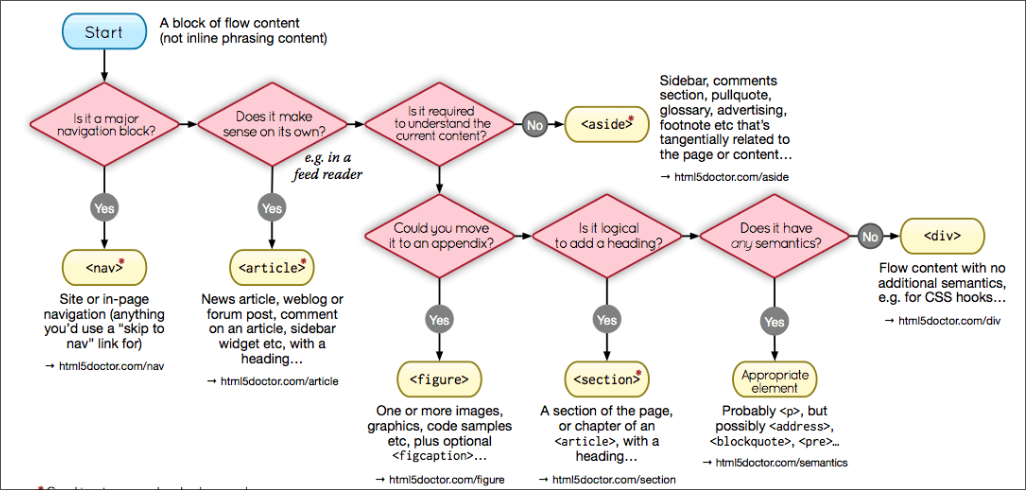
\includegraphics[scale=0.4]{2022-09-27-11:45:58.png}
\section{Global Attritubes}
\begin{tabular}{|p{0,2\linewidth}|p{0.755\linewidth}|}
\hline
accesskey & Specifies a shortcut key to activate/focus an element\\
\hline
class & Specifies one or more classnames for an element (refers to a class in a style sheet)\\
\hline
contenteditable & Specifies whether the content of an element is editable or not\\
\hline
data-* & Used to store custom data private to the page or application\newline
\textcolor{orange}{These (for example) used to handle event bubbling\newline 
data-event= add -> handle add in parent node to rerender, etc\newline
In the parent node you can then perform a check on this by using target.class == add\newline
\textbf{This makes sure you don't use the same function for every single bubbling event!}}\newline
\begin{lstlisting}
document.querySelector("pingpang").addEventListener("click", (event) => { 
  if (event.target.getAttribute("data-eventtype") == "add") {
   rerender();
  } else {
    console.log("pingpang!");
  }
})
\end{lstlisting}
\\
\hline
dir & Specifies the text direction for the content in an element\\
\hline
draggable & Specifies whether an element is draggable or not\\
\hline
hidden &	Specifies that an element is not yet, or is no longer, relevant\\
\hline
id & Specifies a unique id for an element\\
\hline
lang & Specifies the language of the element's content\\
\hline
spellcheck & Specifies whether the element is to have its spelling and grammar checked or not\\
\hline
style & Specifies an inline CSS style for an element\\
\hline
tabindex & Specifies the tabbing order of an element\\
\hline
title & Specifies extra information about an element\\
\hline
translate & Specifies whether the content of an element should be translated or not\\
\hline
\textbf{\emph{Tag Omission}} & You can omit certain tags. Namely the following: <html>, <body>, <head>, <p>, <li>.\newline
It is generally recommended to do this for stylistic reasons.\\
\hline
\end{tabular}
\section{Script in HTML}
\begin{tabular}{|m{0.2\linewidth}|m{0.755\linewidth}|}
\hline
<script> & 
\textcolor{orange}{To use js inside html you need to be sure that the DOM is already loaded}\newline
\begin{lstlisting}
<head>
<!-- the button can't be accessed here! -->
</head>
<body>
<button>clickme</button>
<script> 
// some js script for the button
// make sure to place it here
</script>
</body>
\end{lstlisting}\\
\hline
\end{tabular}
\end{table}
\pagebreak
\begin{table}[ht!]
\section{Web Server}
\begin{tabular}{|m{0.2\linewidth}|m{0.755\linewidth}|}
\hline
Https Request & 
Https uses requests to both get and push data.\newline
We call them \textbf{GET request} and \textbf{POST request}.\newline
Usually we only use GET requests in combination with js like this:\newline
\begin{lstlisting}
async function fetchFromURL() {
  try {
    const response = await fetch('result.json', { method: 'GET'});
    if(response.ok) {
      const content = await response.text();
      console.log(content);
    }
  } catch(e) {
    // erroreroni
  }
}
\end{lstlisting}\\
\hline

\hline

\hline

\hline

\hline

\hline

\hline

\hline

\hline
\end{tabular}
\end{table}
\pagebreak
\begin{table}[ht!]
\begin{tabular}{|m{0.2\linewidth}|m{0.755\linewidth}|}
\hline

\hline

\hline

\hline

\hline

\hline

\hline

\hline

\hline

\hline
\end{tabular}
\end{table}
\end{document}

